\documentclass[a4paper,11pt]{article}

\usepackage[left= 1.5cm,text={18cm, 25cm},top=2.5cm]{geometry}
\usepackage[utf8]{inputenc}
\usepackage[T1]{fontenc}
\usepackage{times}
\usepackage{paralist}
\usepackage{graphicx}
\usepackage{textcomp}
\usepackage{enumitem}
\usepackage{amssymb}
\usepackage{amsmath}
\usepackage{xcolor}
\usepackage[ddmmyyyy]{datetime}
\usepackage{array}
\pagestyle{plain}
\pagenumbering{arabic}
\usepackage[slovak]{babel}


\renewcommand*\contentsname{Obsah}

\newdateformat{mydate}{\twodigit{\THEDAY}.{ }\shortmonthname[\THEMONTH] \THEYEAR}

\pagenumbering{arabic}

\usepackage{url}
\DeclareUrlCommand\url{\def\UrlLeft{<}\def\UrlRight{>} \urlstyle{tt}}

% \usepackage{indentfirst}

\begin{document}
\selectlanguage{slovak}

\begin{titlepage}
\begin{center}
    {\Huge \textsc{Vysoké učení technické v Brně}}
\vspace{\stretch{0.01}}
    
    {\LARGE \uppercase{FAKULTA INFORMAČNÍCH TECHNOLOGIÍ}}
    
\begin{figure}[h]
\vspace{5.0cm}
\centering

\includegraphics[scale=0.15]{logo.png}
\vspace{-10.0cm}
\end{figure}
    
\vspace{\stretch{0.382}}
	{\LARGE Projekt IAL, 2018Z}
\vspace{\stretch{0.02}}

	{\Huge \textbf{Zafarbenie grafu}}
\vspace{\stretch{0.02}}\\

{\LARGE {Projekt č.6}}\\

\begin{figure}[h]
\centering
{\Large {\mydate\today}}
\vspace{6cm}
\end{figure}

\end{center}
\begin{compactitem}
\item[] \textbf{Tím:}
\item[] Adámek Josef, xadame42
\item[] Barnová Diana, xbarno00
\item[] Vanický Jozef, xvanic09
\item[] Weigel Filip, xweige01
\end{compactitem}

\end{titlepage}

\tableofcontents
\newpage

\section{Zadanie}
Vytvoriť program pre hľadanie \textbf{minimálneho zafarbenia neorientovaných grafov.} 
Ak existuje viacero riešení, stačí nájsť iba jedno. Výsledky prezentujte vhodným spôsobom. Súčasťou projektu bude načítavanie grafov zo soúboru a vhodné testovacie grafy. V dokumentácii uveďte teoretickú zložitosť úlohy a porovnejte ju s experimentálnymi výsledkami.

\section{Práca v týme}
\subsection{Príprava a plán}
Pred začiatkom vývoja boli vzaté do úvahy schopnosti každého člena týmu, na základe ktorých boli pridelené úlohy. Časové rámce jednotlivých úloh boli len orientačné pre udržanie prehľadu nad postupom a zvyšným časom do ukončenia projektu. Bol vytvorený privátny repozitár na platforme Git-Hub, fungujúci na technológii Git pre ľahké verzovanie projektu a možnosti vytvoriť jednotlivé vetvy pre každú verziu a nezávislý vývoj a pre prípadnú orientaciu mezi verziami či vrátenia k predchádzjúcej verzii. Pro statickú analýzu kódu sme využili službu Codacy a službu CircleCI pre automatické spúšťanie testov.
\subsection{Postup a rozdelenie práce}
Pri tomto projekte sme sa rozhodli využiť metódu Test-driven development a to z dôvodu zefektivnenia celeho vývoja. Najskôr bol napísaný test k verzii, ktorá bola až následně naprogramovaná. Tak sa zabránilo k zavedeniu chybu do už funkčnej verzii našeho programu.
\subsection{Komunikácia}
Komunikácia v tíme prebiehala prostredníctvom služby Messenger, ale aj osobne na pravidenlých stretnutiach, ktoré sme si naplánovali už na začiatku riešenia projektu.

\section{Teoretická časť}
\subsection{Priblíženie problematiky}
\textbf{Graf} (všeobecne) je definovaný trojicou G=(N, E, I), kde 
\begin{itemize}
    \item N je množina uzlov, ktorým je možné priradiť hodnotu
    \item E je množina hrán, ktorým je možné priradiť hodnotu. Každá hrana spojuje dva uzly a môže byť orientovaná. Ak je hrana orientovaná tak sa hovorí o orientovanom grafe. V našom prípade sa teda jedná o \textbf{neorientovaný graf}, pretože hrany sú neorientované.
    \item I je množina spojenia, ktorá jednoznačne určuje dvojice uzlov daného grafu
\end{itemize}

\begin{figure}[h]
  \centering
  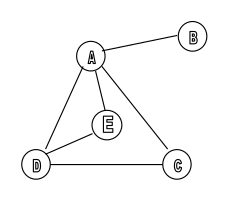
\includegraphics[scale=0.60]{neor_graf.png}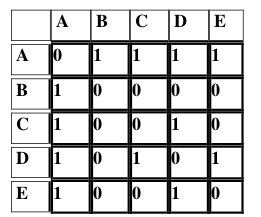
\includegraphics[scale=0.58]{matrix_n_graf.png}
  \caption{Príklad neorientovaného grafu a jeho matice}
  \label{fig:graf}
\end{figure}

\textbf{Implementácia} neorientovaného grafu je pomocou matice koincidencie t.j spojenia. Táto matica je symetrická podľa hlavniej diagonály.

\textbf{Zafarbením grafu} rozumieme priradenie farieb uzlom grafu, pričom žiadne dva susedné uzly nesmú byť zafarbené rovnako. Minimálny počet použitých farieb sa nazýva \textbf{chromatické číslo}. Práve riešenie s týmto chromatickým číslom v našom projekte hľadáme. 
\newpage

\section{Spustenie programu}
./main -f FILENAME [-h] [-b], kde
\begin{itemize}
    \item -f FILENAME určuje názov súboru, ktorý obsahuje maticu grafu
    \item -b je voliteľný parameter,  ktorý spustí "brief mode" programu, takže program vypíše na štandardný výstup iba chromatické číslo spracovaného grafu
    \item -h je voliteľný parameter, ktorý má na starosti vypísať  na štandardný výstup nápovedu pre užívateľa
\end{itemize}

\section{Testovanie projektu}
Pre projekt sme najprv vytvorili menšie testovacie grafy, ktorých chromatické číslo sme vedeli sami určiť. Tie sme neskôr použili pri testovaní správnosti každej novej verzie našeho programu, pomocou nami vytvoreného testovacieho skriptu. Neskôr sme na generovanie grafov vytvorili skript, ktorý dokáže vygenerovať ľubovoľný neorientovaný graf, podľa zadaných parametrov. Testovanie prebiehalo na platforme Ubuntu, MacOS a FreeBSD.

\section{Implementácia}
\subsection{Algoritmus}
Ako prvú metódu pre zafarbenie grafu sme použili metódu slepého prehľadávania so spätným navrátom (angl: backtracking). Pre náš typ problému (constraint satisfaction problem) sme túto metódu vybrali, pretože je \textbf{úplná} a zároveň \textbf{optimálna}. Neskôr sme zistili, že je táto metóda pomalá aj napriek naším pokusom o jej vylepšenie. Z toho dôvodu sme ako druhú použili metódu doprednej kontroly (angl: forward checking), ktorá sa dá chápať ako vylepšená metóda slepého prehľadávania. Metóda doprednej kontroly sa ako metóda "pozerá" dopredu a tým je schopná rýchlejšie odhaliť kombináciu farieb, ktoré nevedú k riešeniu problému. Metóda je tak schopná redukovať stavový strom a vďaka tomu nieje potrebna používať prílišneho spätného navrátenia. Túto metódu sme konkrétne implementovali pomocou rekurzie.

\subsection{Štruktúry}
Dve primárne štruktúry ideálne pre reprezentáciu neorientovaného grafu v programe sú zoznam susedov a matica susednosti. Zvolili sme maticu susednosti a to z dôvodu vhodného formátu načítania grafu zo vstupu do programu, ale aj kvôli následnej práci s týmto grafom.V programe je matica susednosti implementovaná ako jediné pole a to pre rýchlejší prístup do tejto matice.

Pre reprezentáciu samotného uzlu sme si vytvorili štruktúru "Node", ktorá zahrňuje id uzlu, jeho pridelenú farbu a množinu legálnych farieb. Táto množina je dôležitá pre metódu doprednej kontroly. Množiny farieb jednotlivých uzlov sme implementovali pomocou polí typu bool, v ktorých index predstavuje farbu a hodnota true alebo false označuje, či je táto farba pre daný uzol legálna. Takto reprezentované uzly sú potom zoradené v poli typu "Node", pričom ich index a id sú rovnaké, aby bolo možné k uzlom rýchlejšie pristupovať.

\subsection{Analýza zložitosti algoritmu}
Problém minimálneho zafarbenia grafu (angl: k-coloring) je takzvaný "NP-úplný problém, čo vo výsledku znamená, že hľadanie optimálneho riešenia problému má exponenciálnu zložitosť.

Metóda doprednej kontroly má časovú zložitosť $O(m^n)$, pričom $n$ v kontexte problému hľadania chromatického čísla vyjadruje počet uzlov v grafe a $m$ vyjadruje počet farieb. Pretože pri hľadaní chromatického čísla môže byť počet farieb rovnaký ako počet uzlov, je vlastne časová zložitosť $O(n^n)$.

Priložený graf vyjadruje porovanie teoretickej časovej zložitosti algoritmu s našimi experimentálnymi výsledkami.

\enspace
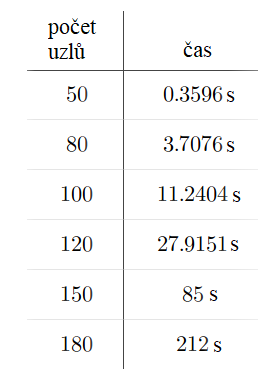
\includegraphics[scale=0.58]{hodnoty.png}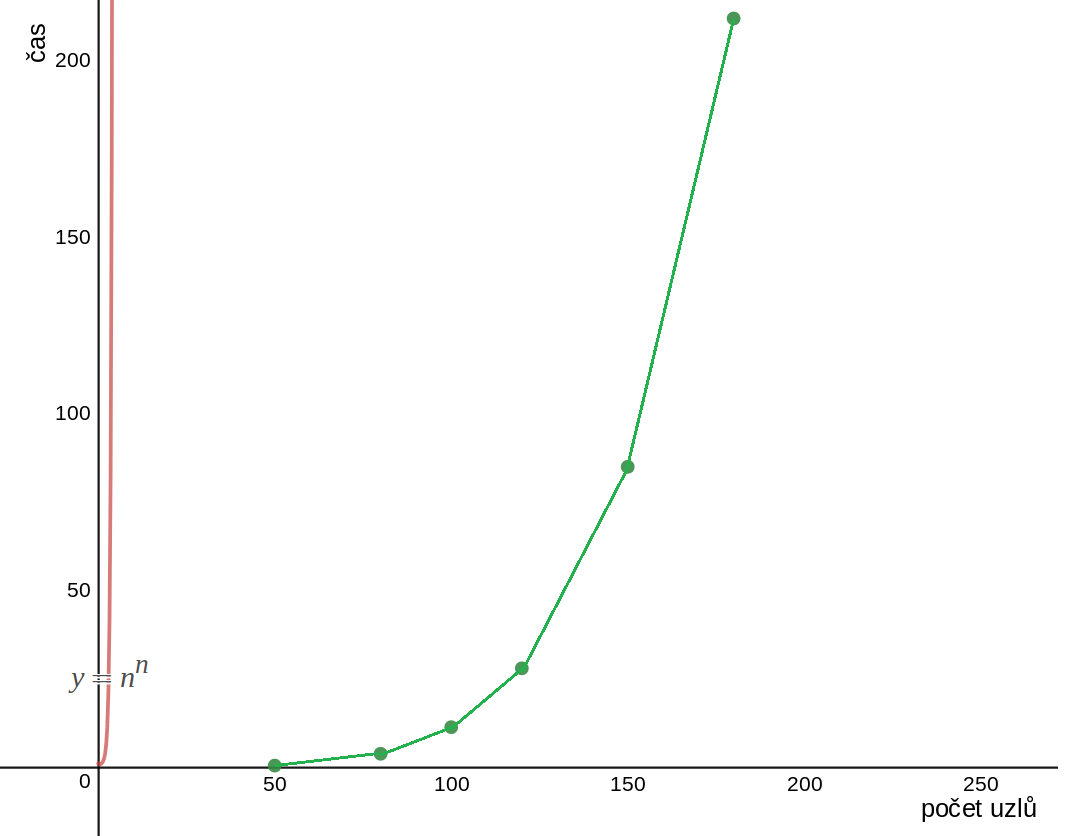
\includegraphics[scale=0.25]{graf_porovnanie.png}

\enspace
Pre stabilitu výsledkov sme použili iba grafy, v ktorých sú spojené všetky uzly so všetkými.
\enspace

\section{Záver}
Sme si vedomí, že aj napriek tomu, že sme sa snažili vytvoriť čo najrýchlejší program pre hľadanie optimálneho riešenia pre hľadanie chromatického čísla v neorientovaných grafoch, existujú ďalšie metódy, ktoré by mohli hľadanie zrýchliť. Jedným z naších pokusov bolo napríklad vylepšiť metódu doprednej kontroly rôznymi heuristikami, avšak kvôli blížiacemu sa termínu odovzdania projektu sme tieto heuristiky nestihli implementovať a odovzdali sme projekt bez nich.

\section{Zdroje}
\begin{compactitem}
\item Opora a prezentácie predmetu IAL
\item Prezentácie predmetu IZU
\item Artificial Intelligence: A Modern Approach (3rd Edition), Peter Norvig, Stuart J. Russell
\item Exponential time algorithms for graph coloring, Uriel Feige, Lecture notes, 2011
\end{compactitem}

\end{document}